\documentclass[conference]{IEEEtran}
\ifCLASSINFOpdf

\newcommand{\redcolor}[1]{\textcolor{red}{#1}}

\newcommand{\figref}[1]{Figure~\ref{#1}}
\newcommand{\secref}[1]{Section~\ref{#1}}
\newcommand{\tabref}[1]{Table~\ref{#1}}
\newcommand{\algoref}[1]{Algorithm~\ref{#1}}

\usepackage{subfig}
\usepackage{caption}
\usepackage{url}
\usepackage{epstopdf}
\usepackage{graphicx}
%\usepackage[pdftex]{graphicx}
% % declare the path(s) where your graphic files are
%\graphicspath{{../figures/}}
%  % and their extensions so you won't have to specify these with
%  % every instance of \includegraphics
%\DeclareGraphicsExtensions{.pdf,.jpeg,.png}
\else
\fi
% *** MATH PACKAGES ***
%
%\usepackage[cmex10]{amsmath}
% *** SPECIALIZED LIST PACKAGES ***
%
\usepackage{algorithmicx}

% *** ALIGNMENT PACKAGES ***
%
%\usepackage{array}
%\usepackage{mdwmath}
%\usepackage{mdwtab}
%\usepackage{eqparbox}
% *** SUBFIGURE PACKAGES ***
%\usepackage[tight,footnotesize]{subfigure}
%\usepackage[caption=false]{caption}
%\usepackage[font=footnotesize]{subfig}

% *** FLOAT PACKAGES ***
%
%\usepackage{fixltx2e}
%\usepackage{stfloats}
% *** PDF, URL AND HYPERLINK PACKAGES ***
%\usepackage{url}
% correct bad hyphenation here
\hyphenation{op-tical net-works semi-conduc-tor}


\begin{document}
%
% paper title
% can use linebreaks \\ within to get better formatting as desired
\title{Back to Basics: Simplifying Non-Intrusive Appliance Load Monitoring Using Combinatorial Optimization}


% author names and affiliations
% use a multiple column layout for up to three different
% affiliations
\author{\IEEEauthorblockN{Author1}
\IEEEauthorblockA{Indraprastha Institute of Information Technology\\
India\\
}
\and
\IEEEauthorblockN{Author2}
\IEEEauthorblockA{Twentieth Century Fox\\
Springfield, USA\\
Email: homer@thesimpsons.com}
\and
\IEEEauthorblockN{James Kirk\\ and Montgomery Scott}
\IEEEauthorblockA{Starfleet Academy\\
San Francisco, California 96678-2391\\
Telephone: (800) 555--1212\\
Fax: (888) 555--1212}}
% make the title area
\maketitle


\begin{abstract}
%\boldmath
Non-Intrusive appliance load monitoring (NIALM) is the process of disaggregating the overall electricity usage into constituent appliances. In this paper we extend the Combinatorial Optimization (CO) approach for disaggregation, which was originally proposed in the seminal work on NIALM, in following two ways: 1) Breaking the problem into subproblems and reducing the state space; 2) Applying additional constraints backed by sound domain expertise. We evaluate our approach using REDD dataset and show practical problems which need to be solved while dealing with the dataset. We also propose a metric for evaluating NILM, which we believe overcomes many shortcomings of commonly used metrics.
\end{abstract}
\IEEEpeerreviewmaketitle



\section{Introduction}
% no \IEEEPARstart
\begin{itemize}
\item Motivate the importance of energy consumption in building
\item Motivate that appliance level information is crucial - detailed feedback and optimized decision making \cite{darby}
\item Challenges with getting appliance level information - introduce NIALM~\cite{hart}
\item introduce your proposed approach
\item Enumerate the contributions
\end{itemize}

Primary contributions of our work are:
\begin{itemize}
\item Fill it up with 2-3 crisp points
\end{itemize}
Open source implementation of the proposed work is released for comparative analysis with other NIALM approaches as an IPython notebook\footnote{\url{http://www.ipython.org}}. We believe this is the first extensive release of a generic NIALM

\section{Related work}
NIALM has been well studied in the recent past and survey papers \cite{survey1,survey2,survey3} present its classification across various dimensions. Following are three important classification dimensions:
\begin{itemize}
\item \textbf{Frequency of data collection}: Approaches such as harmonic analysis require data to be sampled at more than a thousand samples a second. Whereas approaches 
\item \textbf{Supervised/Unsupervised}: 
\end{itemize}
When you do the comparison, bring up how is your work different rather than just saying X did A and Y did B.
\begin{itemize}
\item Classification of different NIALM approaches - High/Low frequency, Time/Frequency domain analysis, supervised/unsupervised~\cite{survey1,survey2,survey3}.

For a more detailed overview the reader is referred to the above mentioned survey papers.

\item Discuss the modeling approaches that are used
\begin{itemize}
\item Additive Factorial HMM
\item Difference HMM \cite{parson2012_aaai}
\end{itemize}

\item Datasets used: Recent datasets have spurred this field
\begin{itemize}
\item REDD \cite{redd}
\item Blued \cite{blued_cmu}
\item Smart* \cite{smart}
\end{itemize}

\end{itemize}


\section{NIALM}
Discuss in brief the NIALM problem
\subsection{Terminologies/ Notations}
Borrow the notation used by Parson and Hart.
\begin{itemize}
\item Time slice: $t\in {1,..T}$
\item Appliance: $n\in{1,..N}$
\item Input: Aggregate power sequence: $x=\{ x_1,..,x_T\}$
\item Input: Ground truth power sequence for each appliance: $\theta^n=\{\theta_1^n,...,\theta_T^n\}$
\item Infer: Power draw by constituent appliance: $y^n=\{y_1^n,..y_T^n\}$
\item Each appliance has $K$ (from k=1 to K )states and consumes $\mu_k$ power corresponding state
\item Appliance state: $z^n=\{z_1^n,..z_T^n\}$ where  $z_i^n \in [1,..K]$ Also $z_{i,k}^n$ denotes whether $n^{th}$ appliance is in $k^{th}$ state at time $i$.
\end{itemize}

\subsection{NIALM using combinatorial optimization}
This approach resembles subset sum problem and tries to minimize the difference of total observed power from the sum of various possible subsets coming from various combinations of appliances in different states. For each appliance we assume \textbf{K} states and at a given time, an appliance can only be in a single state. This is given as: 
$z_{t,k}^n\in\{0,1\} $ and, $$\sum\limits_{k=1}^{k=K} z_{t,k}^n=1$$The power drawn by $n^{th}$ appliance in $k^{th}$ state is given by:
$$\mu^n=\{\mu_1^n,..\mu_K^n\}$$ Thus, CO can be formulated as:
$$z_t=arg min_{z_t}|x_t-\sum\limits_{n=1}^{N}\sum\limits_{k=1}^{K}z_{t,k}^n\mu_k^n|$$
Correspondingly the power draw by $n^{th}$ appliance is given by: $y^n=\{\mu_{z_1^n}^n,..\mu_{z_T^n}^n \}$

\begin{itemize}
\item Statespace is $K^N$
\item We assign different loads to different mains, $N_i$ loads to $Mains_i$, $\sum\limits_{1}^{p}{N_i}=N$. Now different state spaces are
$K^{N_1}$.... We can define the overall state space as $\max{K^{N_i}}$

As a practical example, two mains, 20 appliance, state space before = $2^{20}$. After = $2^{10}$. Exponential reduction in state space.
\end{itemize}

Highlight what is the simplification you are bringing forth.

\section{Divide and Conquer NIALM (DaCo-NIALM)}
\begin{figure}
\centering 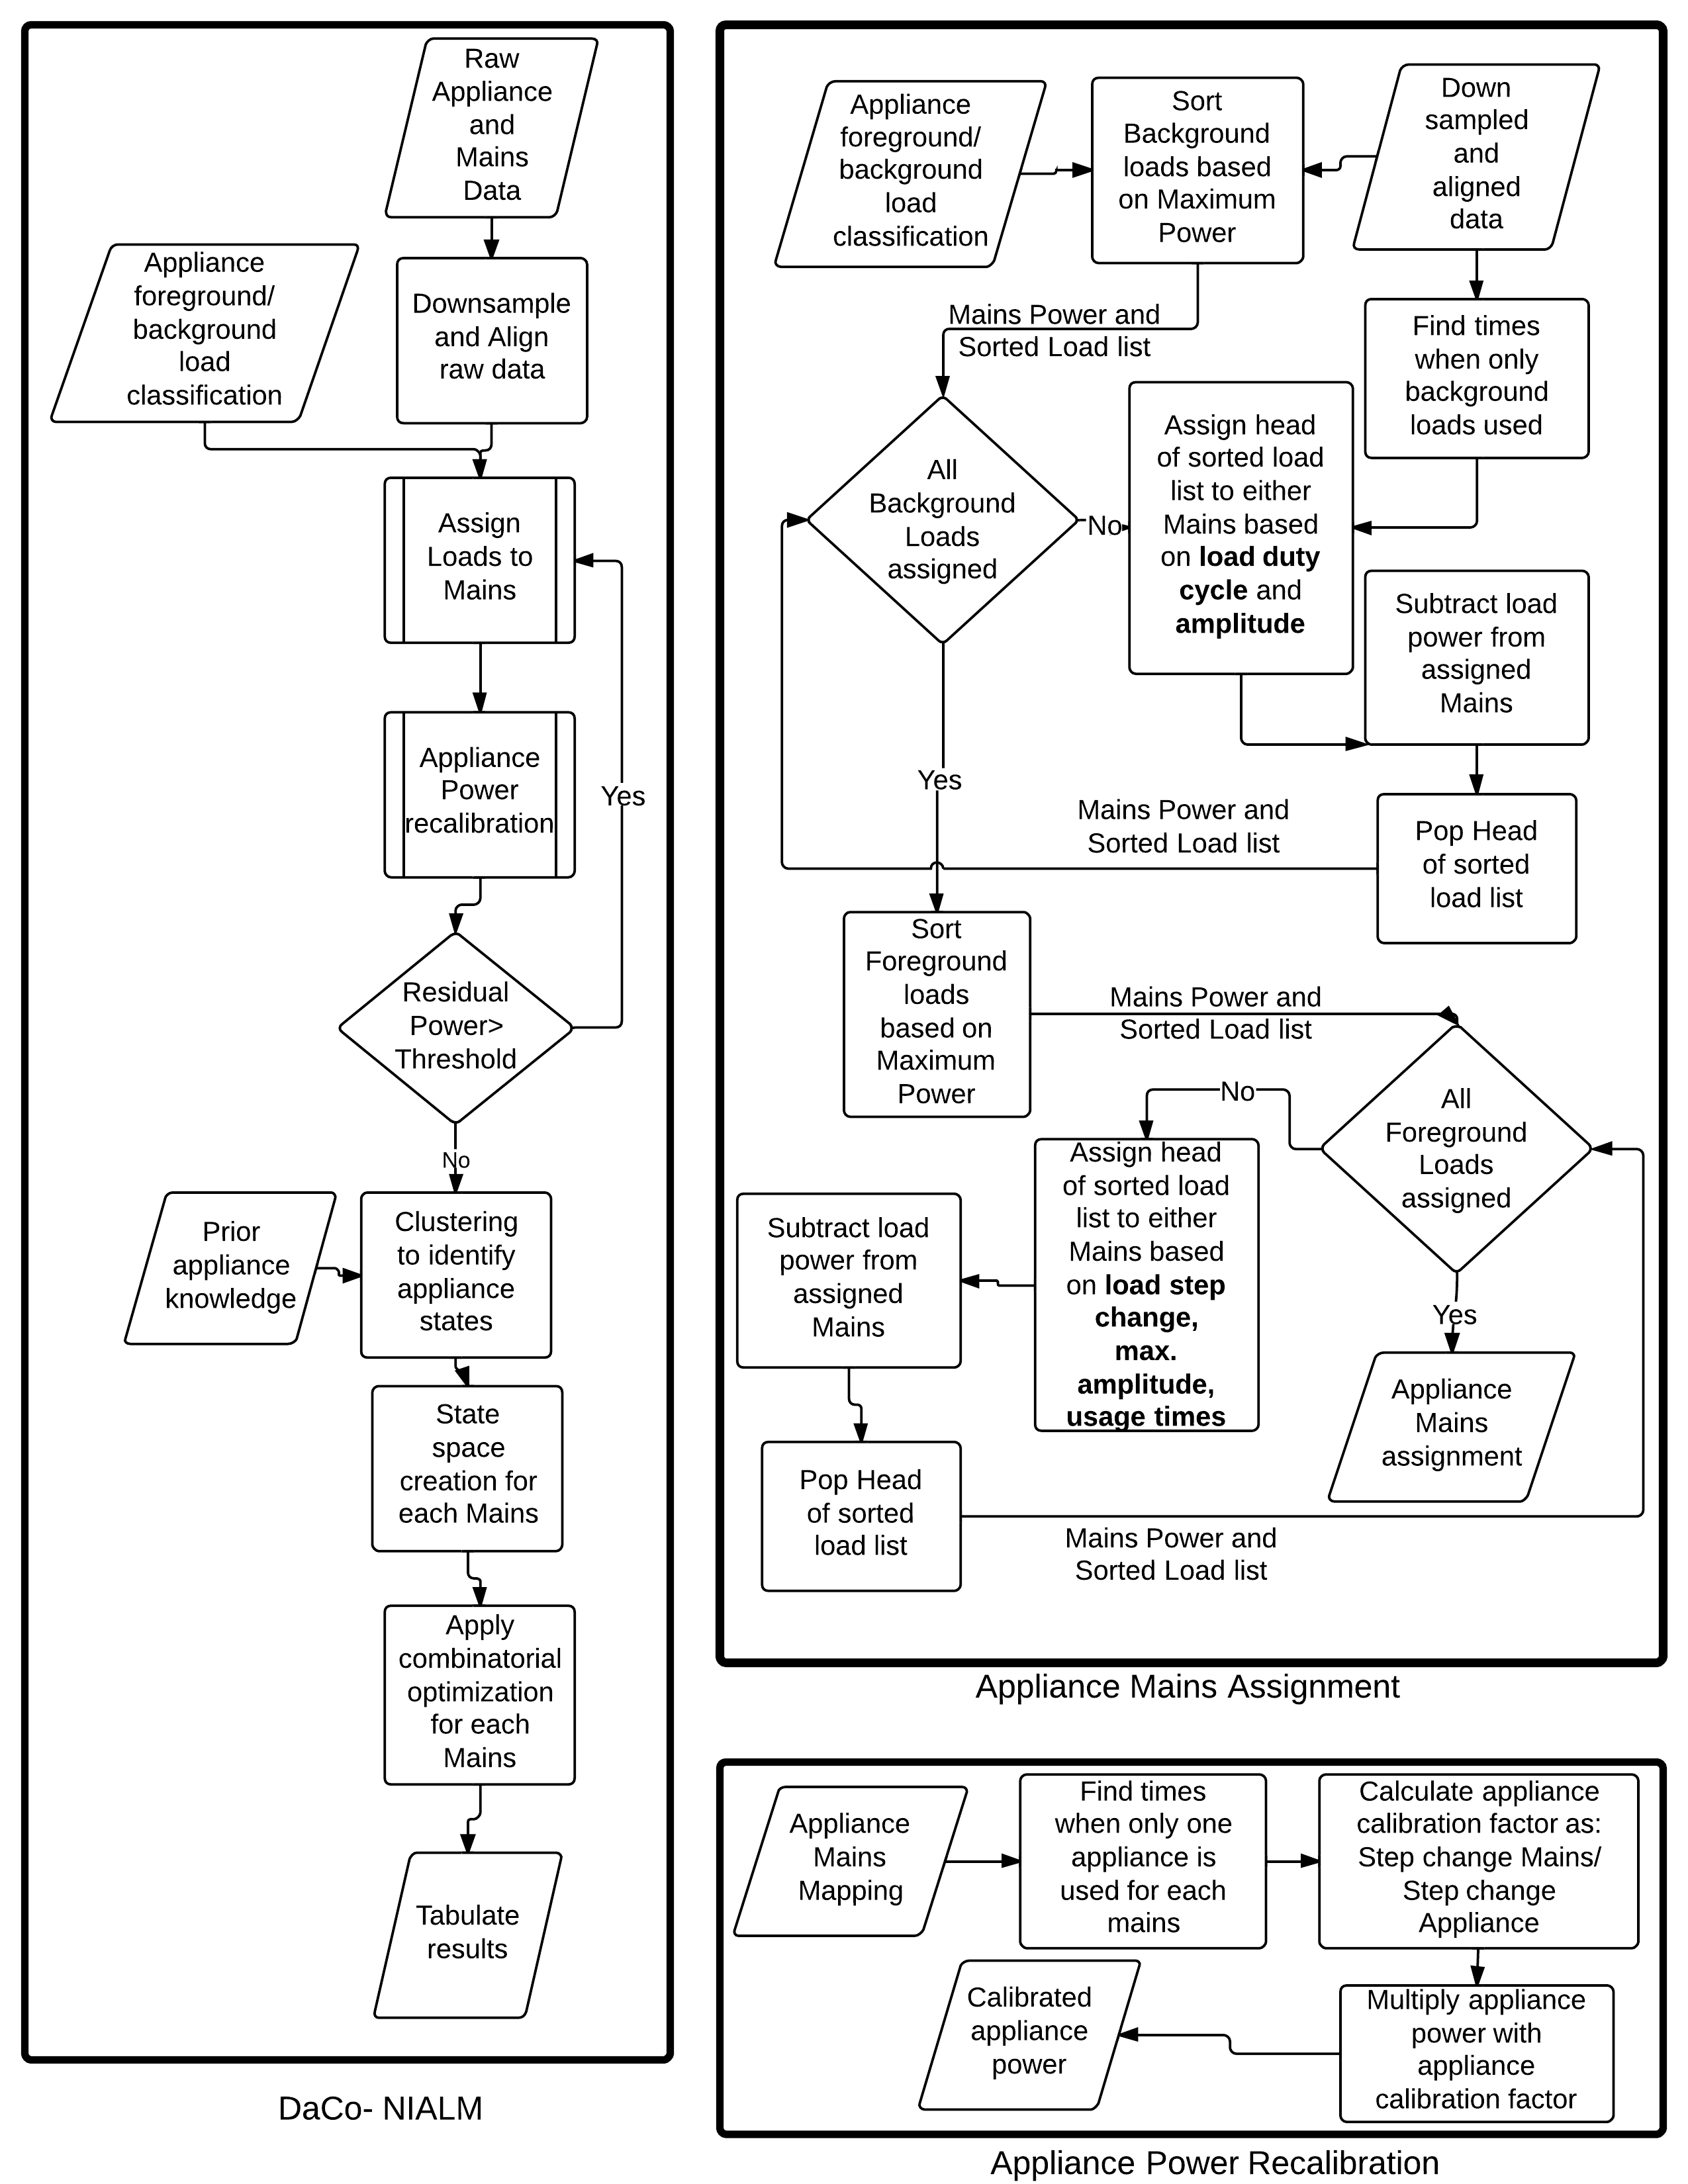
\includegraphics[scale=0.1]{./figures/algo_3.png}
\caption{Divide and Conquer NIALM}
   \label{fig:algorithm}
\end{figure}
In this section we explain the various steps involved in DaCo-NIALM which is shown in \figref{fig:algorithm}.
\begin{enumerate}
\item \textbf{Downsample and align raw data}: While performing Combinatorial Optimization it is desired that transients and fluctuations in the power signal are filtered. The transients occur due to the high starting current of the appliance, whereas the fluctuations are a consequence of minor voltage fluctuations and oscillatory nature of loads. \figref{fig:downsample_startup} and \figref{fig:downsample_voltage} show how starting current and voltage fluctuations can be filtered by downsampling. 
%To overcome these we downsampled our data to one minute resolution using mean filter. 
Further realignment amongst the appliance level data and mains level data is needed owing to different frequency of data collection and missing data.
\begin{figure} 
	
    \subfloat[\scriptsize Filtering startup transients]{
    \label{fig:downsample_startup}
    \includegraphics[scale=0.1]{./figures/downsampled_1.png}}
    \subfloat[\scriptsize Filtering voltage fluctuations and oscillations]{
        \label{fig:downsample_voltage}
        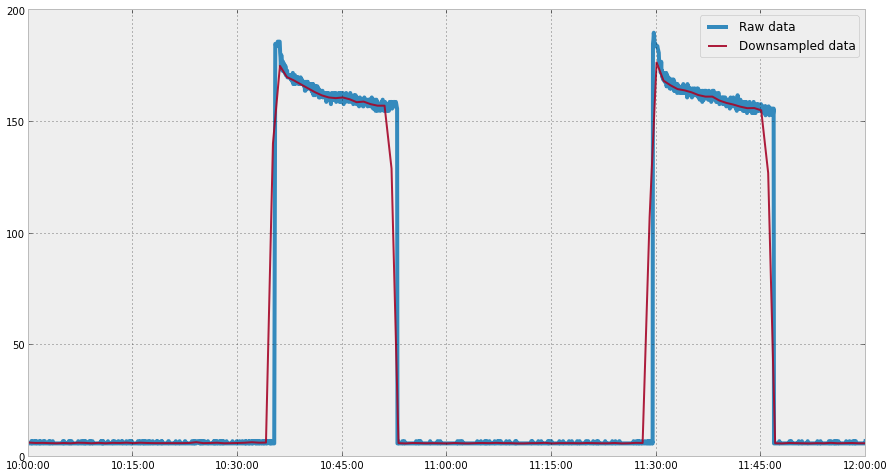
\includegraphics[scale=0.1]{./figures/downsampled_2.png}}
  	\caption{Effect of downsampling appliance data}
    \label{fig:downsampling}
\end{figure}

\item \textbf{Assigning Loads to Mains}: This is the most important step of the algorithm and aims to identify the mapping between appliances and mains. Based on domain expertise we label the appliances in a home into background (loads which run independently throughout the day without user interference) such as refrigerator, and foreground (loads which are highly correlated with human usage) such as stove. Background loads are easier to detect since they are ON even during periods of low human activity such as night time. Thus, we first aim to assign background loads to different mains. Loads with higher mean power consumption are easier to identify and thus we sort background loads based on mean power in descending order. Starting from the head of this list (appliance having highest mean power consumption) we iteratively attempt to do its assignment and once assign subtract this load from assigned mains to make further analysis easier. As a first check we see if the mean power of the appliance is greater than mean power of any mains for all time instances. If so, we can safely assign the appliance to the other mains. If this step is unable to provide conclusive evidence we look at the periodicity associated with such background loads during periods of low or no human activity (such as night time). \figref{fig:assignment_1} shows how based on refrigerator duty cycle it is mapped to Mains 2. On similar lines assignment of foreground loads can be done. \figref{fig:assignment_2} shows assignment of dishwasher to Mains 1, which is easy to do, since during this time window, mean dishwasher power is greater than mean Mains 2 power.
\begin{figure} 
	
    \subfloat[\scriptsize Assigning based on duty cycle]{
    \label{fig:assignment_1}
    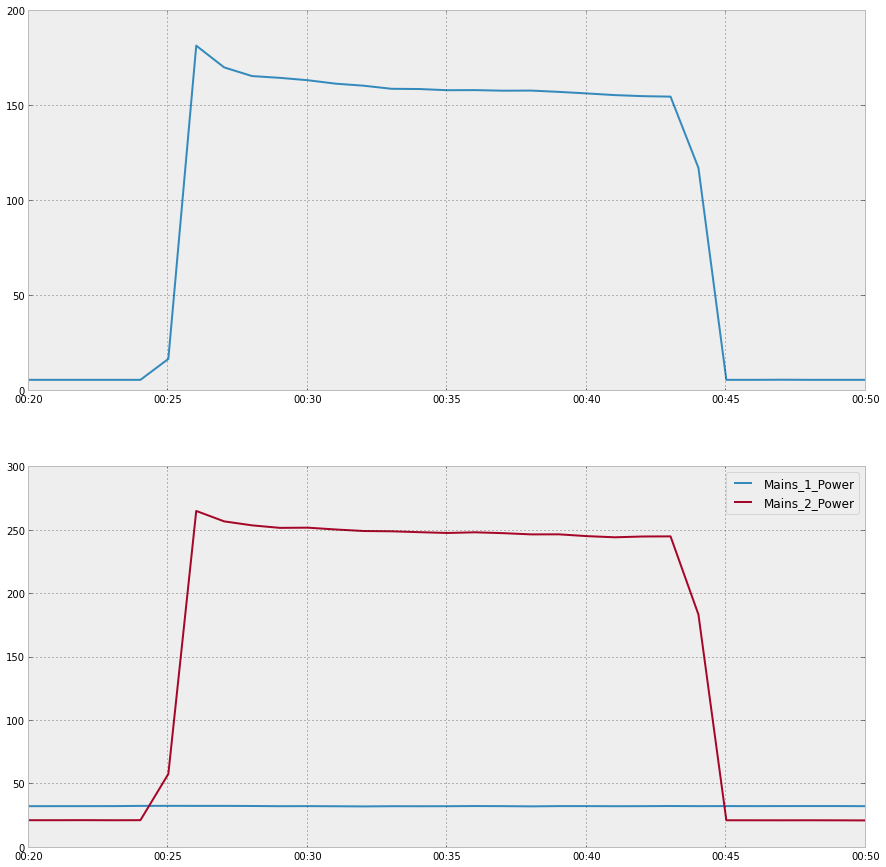
\includegraphics[scale=0.1]{./figures/assignment_1.png}}
    \subfloat[\scriptsize Assigning based on power threshold and step change times]{
        \label{fig:assignment_2}
        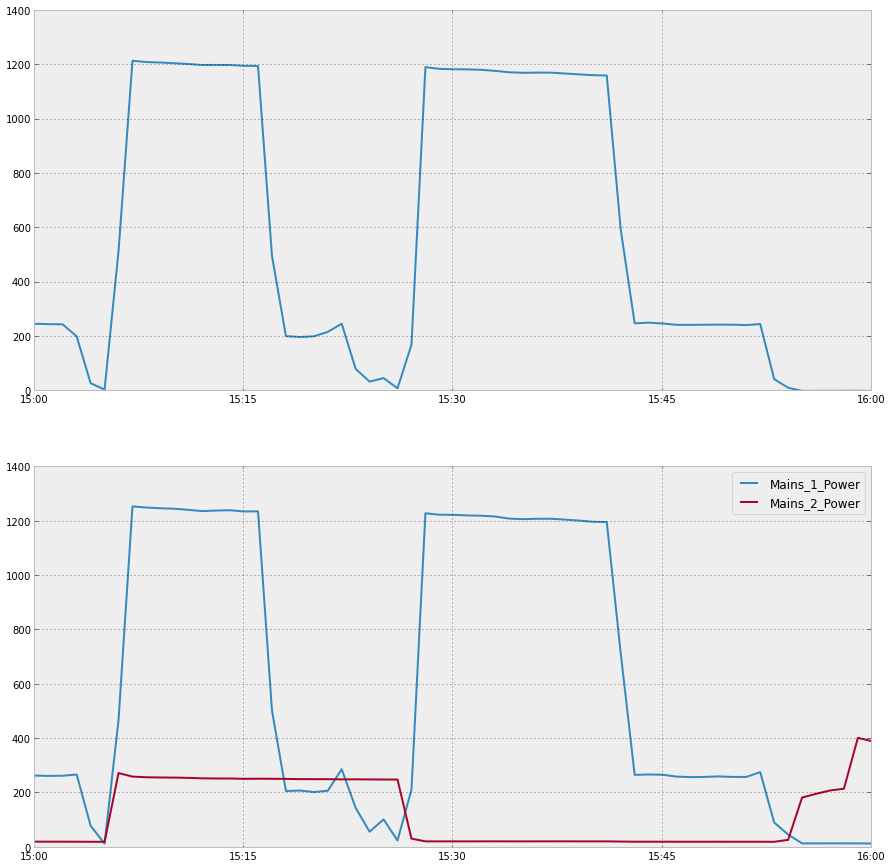
\includegraphics[scale=0.1]{./figures/assignment_2.png}}
  	\caption{Assigning Refrigerator and Dishwasher to Mains 2 and Mains 1 respectively}
    \label{fig:assignment}
\end{figure}

\item \textbf{Appliance Power Recalibration}: Since different hardware is used for measuring appliance and mains data there may be a need to calibrate the two. Since mains data is usually collected using better precision hardware, we keep mains data as a reference and calibrate appliance data against it. In practice we found appliance level monitors to usually provide only real power whereas the mains monitors can provide much more like reactive and active power. Like the previous step, time instances when an appliance in a particular mains is single used are identified. The ratio of mains and appliance power step changes occurring this window serve as the calibration factor for that appliance. Further each appliance power is corrected with the corresponding calibration factor.

\item \textbf{Clustering to identify appliance states}:
\begin{enumerate}
\item Step changes occurring in Mains vs Appliances
\item Isolating single appliance usage
We use \cite{kmeansplusplus} to run our clustering
\end{enumerate}
\item Appliance states identification using clustering (Possibly talk about unbalanced data, but leave it for future work)
\item State space creation
\item Applying CO for different mains
\item Find energy distribution by appliance and assign weights (To be used in results)

\end{enumerate}





%\begin{figure*}[!t]
%\centerline{\subfloat[Case I]\includegraphics[width=2.5in]{downsampled_1}%
%\label{fig_first_case}}
%\hfil
%\subfloat[Case II]{\includegraphics[width=2.5in]{subfigcase2}%
%\label{fig_second_case}}}
%\caption{Simulation results}
%\label{fig_sim}
%\end{figure*}

\subsection{Load assignment}
Draws inspiration from work by Parson et. al \cite{parson2012_aaai}. From prior knowledge we divide the loads into two different categories: Periodic such as refrigerator and non periodic such as Television.

\section{Evaluation}
\subsection{About Dataset}

We use REDD dataset \cite{redd} for validating our algorithms. This dataset contains power and voltage data for mains (2 phases) as well as appliances from 6 homes in Boston area collected in the summer of 2011. The data is made available as raw, high frequency (sampled at 15 KHz) and low frequency (Mains at 1 Hz, appliances at ~.3 Hz). Considering the practical implications of residential smart meter installation, we believe that low frequency data represents the most realistic scenario and thus we use this data for analysis. \figref{fig:breakdown} shows 6 hourly breakdown of energy consumption across the different mains in Home 2 .


\begin{figure} 
	
    \subfloat[\scriptsize Mains 1]{
    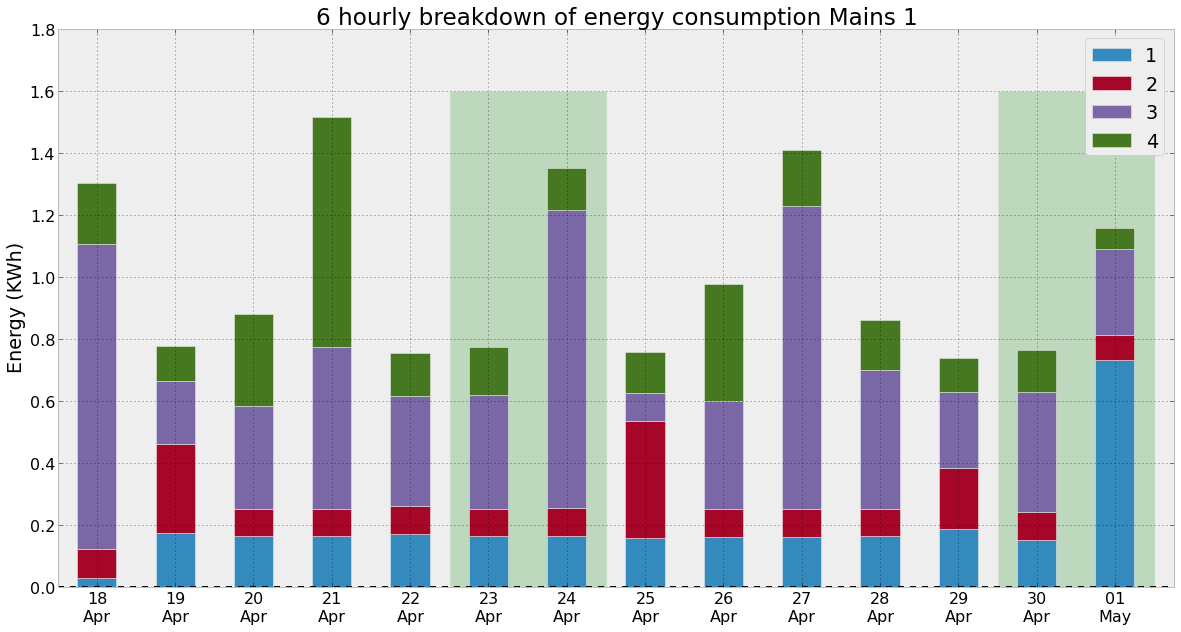
\includegraphics[scale=0.1]{./figures/mains_1_6hr.png}}
    \subfloat[\scriptsize Mains 2]{
        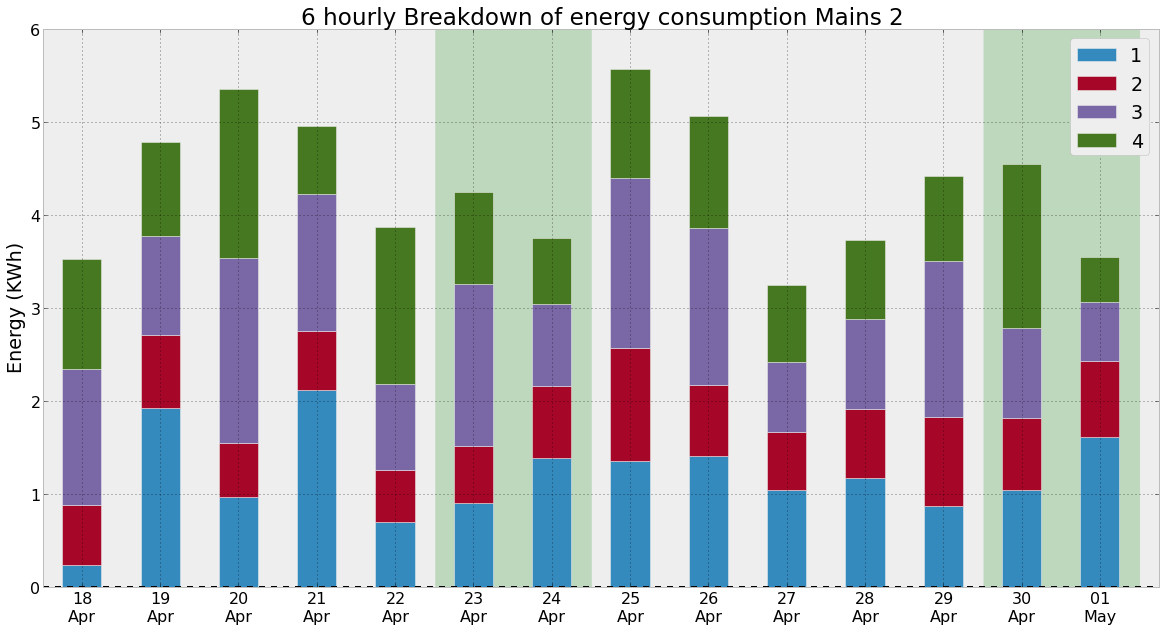
\includegraphics[scale=0.1]{./figures/mains_2_6hr.png}}
  	\caption{6 hourly energy usage breakdown Home 2}
    \label{fig:breakdown}
\end{figure}

\subsection{Evaluation Metric}

Commonly used metrics such as accuracy, sensitivity and specificity can be misleading when applied to NIALM. It can be seen from \figref{fig:confusion} that since stove is mostly in state 0 (Off), accuracy will be largely decided by accuracy for this state, which is misleading, since it is easy to predict off states of appliances irrespective of the approach. Armel et. al \cite{survey1} discuss the lack of a common metric while comparing NIALM approaches. We use the following metrics which have been used in the past work \cite{parson2012_aaai,redd} and were also suggested by Hart \cite{hart}:
\begin{itemize}
\item \textbf{Mean Normalized Error (MNE \%)}: Normalized error in the energy assigned to an appliance over the test period, given by 
$$\frac{|\sum\limits_{t=1}^{T}\theta_t^n- \sum\limits_{t=1}^{T}y_t^n|}{\sum\limits_{t=1}^{T}\theta_t^n} $$
Lesser is better

\item \textbf{RMS Error (RE Watts)}: RMS error per time slice given by
$$\sqrt{\frac{1}{T}\sum\limits_{t=1}^{T}(\theta_t^n-y_t^n)^2}$$
Lesser is better
\item Explain why the metric used by MIT REDD people will fail under some cases
\end{itemize} 
\begin{figure}
\centering 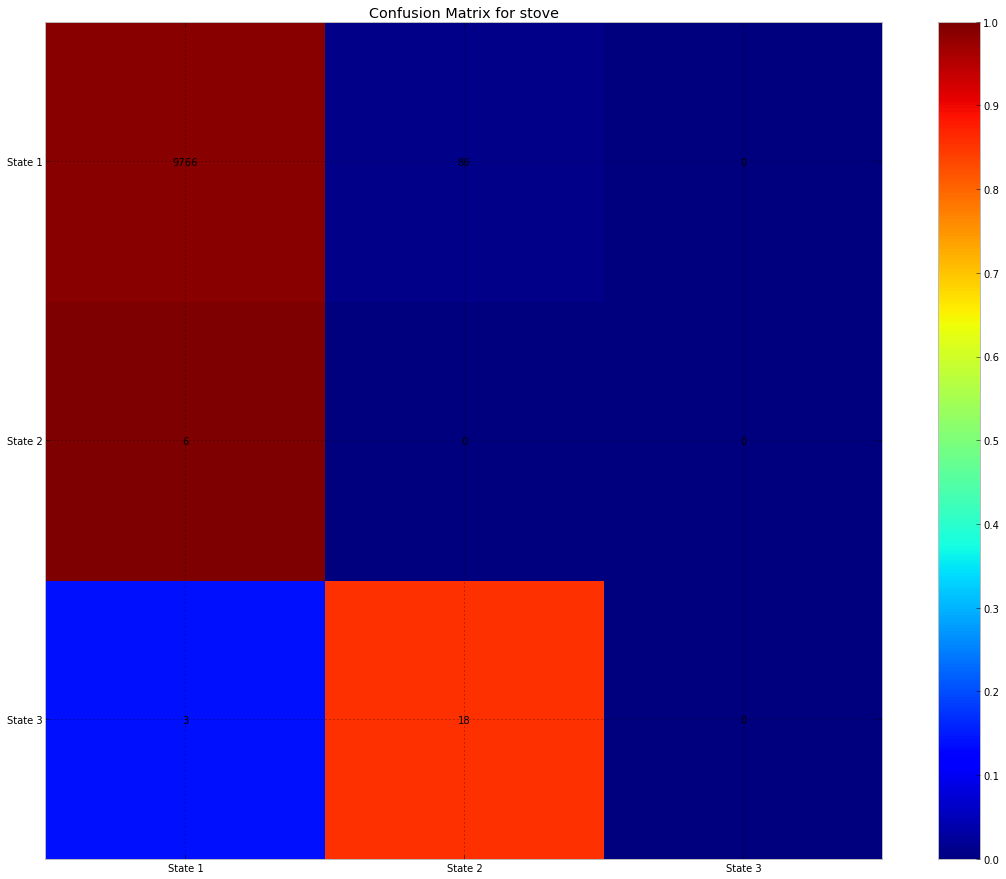
\includegraphics[scale=0.2]{./figures/confusion_stove.png}
\caption{Confusion Matrix showing predicted state accuracy for Stove}
   \label{fig:confusion}
\end{figure}



\subsection{Empirical Analysis}
We analyze data from Home 2 of the REDD dataset and believe that the same analysis can be easily repeated across multiple homes. 
\begin{itemize}
\item Train on first 7, test on last 7 days
\item State assignment, Mains assignment in \tabref{tab:calibration_factors}
\item Overall results in \tabref{tab:results}, first column NILM without dividing into mains and without recalibration, last column with DiCaCo NIALM. Vast reduction in R.E. and M.N.E , especially for most appliance contributing most like refrigerator and lighting	
\item Confusion matrix showing a large improvement in refrigerator recognition in \figref{fig:confusion_ref}
\end{itemize}

\begin{figure} 
	
    \subfloat[\scriptsize Without applying DiCaCo]{
    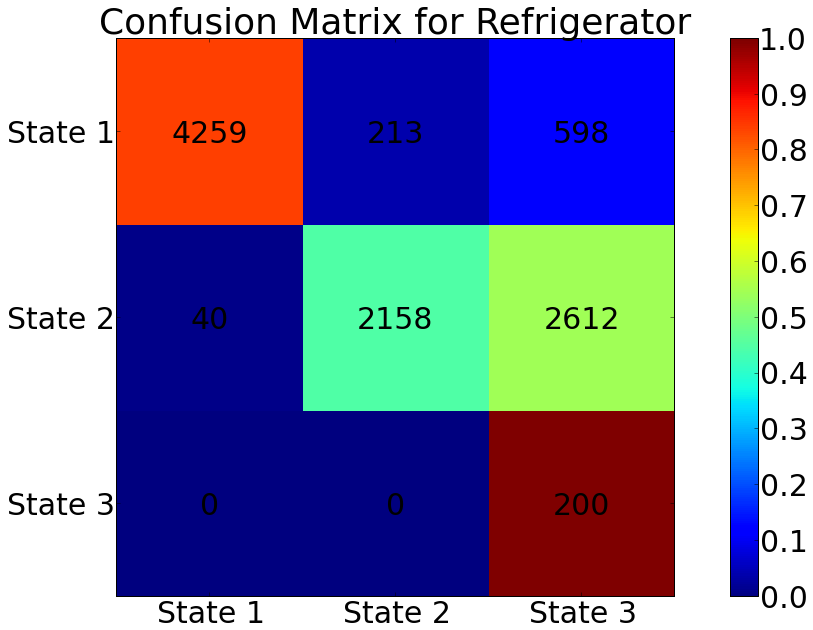
\includegraphics[scale=0.15]{./figures/confusion_before_dicaco.png}}
    \subfloat[\scriptsize After applying DiCaCo]{
        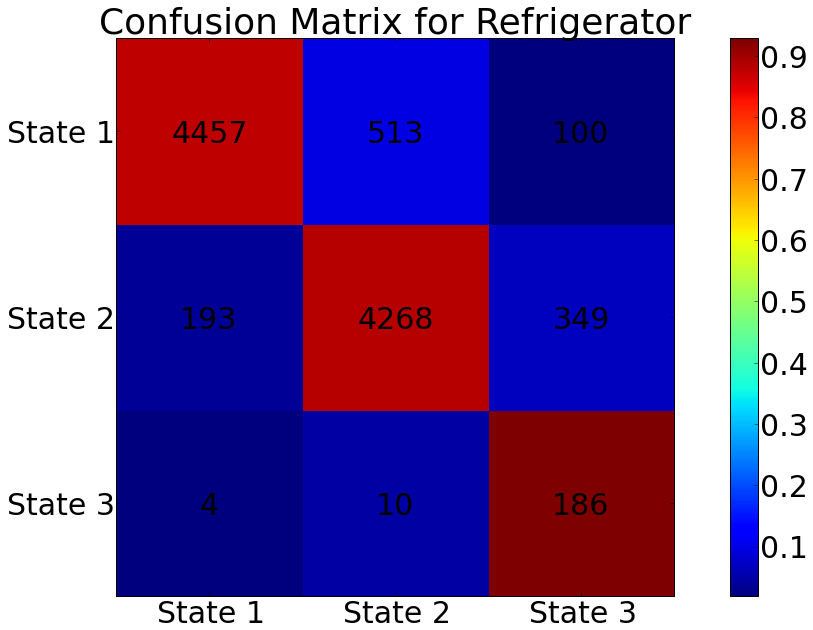
\includegraphics[scale=0.15]{./figures/confusion_after_dicaco.png}}
  	\caption{Confusion Matrix for refrigerator disaggregation}
    \label{fig:confusion_ref}
\end{figure}

%\item Table on Calibration factors
\begin{table}
%%% increase table row spacing, adjust to taste
%%\renewcommand{\arraystretch}{1.3}
%% if using array.sty, it might be a good idea to tweak the value of
%% \extrarowheight as needed to properly center the text within the cells
\caption{Calibration Factors, Mains Assignment and States}
\label{tab:calibration_factors}
%\centering
%%% Some packages, such as MDW tools, offer better commands for making tables
%%% than the plain LaTeX2e tabular which is used here.
\begin{tabular}{|c|c|c|c|}
\hline
Appliance & Mains & States Power (W)& States Power (W)\\
\hline
&&Pre calibration&Post calibration\\
\hline
Refrigerator & 2& 7,162,423 & 9,210,423\\
Microwave &2& 10,832,1730& 10,832,1730\\
Lighting & 2& 9,96,156&10,110,178\\
Dishwasher & 1& 0,256, 1195 & 0,256, 1195\\
Stove& 1 & 0,374& 0,374\\
Kitchen & 1& 5,727&5,727\\
Kitchen 2&1 & 1,204,1032&1,204,1032 \\
%
%
\hline
%
\end{tabular}
\end{table}

\begin{table}
\caption{Mean Normalized Error and RMS error with and without DiCaCo NIALM}
\label{tab:results}
\begin{tabular}{|p{30pt}|p{12pt}|p{14pt}|p{12pt}|p{14pt}|p{12pt}|p{14pt}|p{12pt}|p{14pt}|}
\hline
&\multicolumn{4}{|c|}{Without}&\multicolumn{4}{|c|}{With}\\
&\multicolumn{4}{|c|}{Recalibration}&\multicolumn{4}{|c|}{Recalibration}\\
\hline
&\multicolumn{2}{|c|}{Without Load}&\multicolumn{2}{|c|}{With Load}&\multicolumn{2}{|c|}{Without Load}&\multicolumn{2}{|c|}{With Load}\\
&\multicolumn{2}{|c|}{Division}&\multicolumn{2}{|c|}{Division}&\multicolumn{2}{|c|}{Division}&\multicolumn{2}{|c|}{Division}\\
\hline

Appliance &R.E.&M.N.E.& R.E.&M.N.E.&R.E.&M.N.E.&R.E.& M.N.E.\\
&Watts&\%&Watts&\%&Watts&\%&Watts&\%\\
\hline
Refrigerator & 136 &109 & 71 & 32 & 130 &95  &59 &21\\
Microwave    & 102 &98  & 97 & 110& 104 &97  &96 &109\\
Lighting     & 51  &164 & 48 & 195& 44  &83  &38 &60\\
Dishwasher   & 406 &2947& 63 & 100& 377 &2517&63 &100\\
Stove        & 77  &1191& 36 & 281& 75  &1118&36 &281\\
Kitchen      & 64  &182 & 58 & 168& 69  &196 &58 &168\\
Kitchen 2    & 95  &267 & 91 & 117& 92  &230 &91 &117\\
\hline
Overall      &478  &187 &161 &  58& 450 &157 &168&39\\

\hline

\end{tabular}
\end{table}





\section{Conclusion}
The conclusion goes here.
We also provide mains load assignment of all 6 homes from REDD to further the research in this direction.

\section{Future Work}
\begin{itemize}

\item Applying model on noisy datasets
\item 2 D CO (when Real and Reactive Power are known)
\item Factoring in Time of Day etc.
\item Factoring in Appliance Correlation
\item Factor in switch continuity, essentially leads to Factorial HMM
\item Distributed NILM
\item Adaptive Learning
\end{itemize}

\section*{Acknowledgment}
The authors would like to thank TCS Research and Development for supporting the first author through PhD. fellowship. We would also like to thank NSF- DEITy for funding the project.
\bibliographystyle{IEEEtran}
\bibliography{IEEEabrv,references}

\end{document}


